\documentclass[11pt]{article}
\author{Aimee Barciauskas, Felix Gutmann, Guglielmo Pelino, Thomas Vicente}
\title{Text Mining Homework - Week 3}
\usepackage{tikz}
\usetikzlibrary{fit,positioning}
\usepackage[labelfont=bf]{caption}
\usepackage{amsbsy}
\nofiles

\begin{document}
\maketitle
\pagebreak
\section*{Exercise 2}	

\subsection*{(a)}

\begin{figure}[!htb]
\centering
	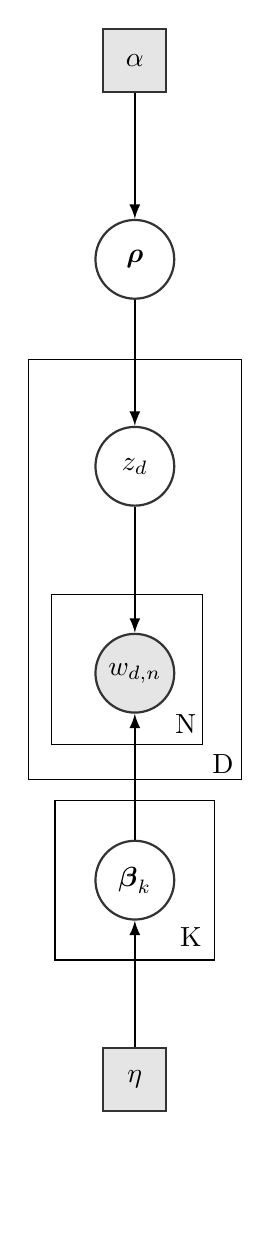
\begin{tikzpicture}
\tikzstyle{main}=[circle, minimum size = 10mm, thick, draw =black!80, node distance = 16mm]
\tikzstyle{rect}=[rectangle, minimum size = 8mm, thick, draw =black!80, node distance = 16mm]
\tikzstyle{connect}=[-latex, thick]
\tikzstyle{box}=[rectangle, draw=black!100]
  \node[rect, fill = black!10] (alpha) [label=center:$\alpha$] { };
  \node[main] (rho) [below=of alpha,label=center:$\boldsymbol{\rho}$] { };
  \node[main] (z) [below=of rho,label=center:$z_d$] {};
  \node[main, fill = black!10] (w) [below=of z,label=center:$w_{d,n}$] { };
  \node[main] (beta) [below=of w,label=center:$\boldsymbol{\beta}_k$] { };
  \node[rect,fill = black!10] (eta) [below=of beta,label=center:$\eta$] { };
  \path (alpha) edge [connect] (rho)
        (rho) edge [connect] (z)
        (z) edge [connect] (w)
        (eta) edge [connect] (beta)
        (beta) edge [connect] (w);
  \node[rectangle, inner sep=0mm, fit= (z) (w),label=below right:N, yshift=-12mm,xshift=-1.3mm] {};
  \node[rectangle, inner sep=8.4mm,draw=black!100, fit= (z) (w)] {};
  \node[rectangle, inner sep=4.4mm,draw=black!100, fit= (w),label=below right:D,xshift=-1mm,yshift=0.5mm] {};
 % \node[rectangle, inner sep=4.6mm, fit= (z) (w),label=below right:M, xshift=12.5mm] {};
  %\node[rectangle, inner sep=9mm, draw=black!100, fit =  (z) (w)] {};
   %\node[rectangle, inner sep=4.4mm,draw=black!100, fit= (beta)] {};
  \node[rectangle, inner sep=5mm,draw=black!100,fit= (beta)] {};
  \node[rectangle, inner sep=0mm,fit= (rho) (beta),label=below right:K, yshift=-39mm,xshift = -2] {};
\end{tikzpicture}
\caption{DAG Representation}
\end{figure}

\pagebreak
\subsection*{(b)}

The \textit{Markov Blanket} of node $V_i$ in the DAG consists of its parents, its children and the parents of its children. Applying this definition table (1) shows the Markov Blanket for the model.\\

\begin{table}[!htb]
\centering
\begin{tabular}{ l | c  }
	\textbf{Node} & \textbf{Nodes in Markov Blanket} \\
	\hline
	$w_{d,n}$ & $\boldsymbol{\beta}_k$, $z_d$  \\
	$z_d$& $w_{d,n}$, $\boldsymbol{\beta}_k$  \\
	$\boldsymbol{\beta}_k$&$w_{d,n}$, $z_d$, $\boldsymbol{\beta}_{-k}$
\end{tabular}
\caption{Markov Blanket}
\label{table:tab1}
\end{table}

\subsection*{(c)}

\begin{enumerate}
	\item Choose values for $\alpha$ and $\eta$
	\item For s $\in$ $\{1,\dots,S\}$: 
	\item[-] sample from $\textbf{P}\bigg[\boldsymbol{\rho}^s\bigg|z_d^{(s-1)}\bigg] \propto \textbf{P}\bigg[z_d^{(s-1)}\bigg|\boldsymbol{\rho}^s\bigg]\textbf{P}\bigg[\boldsymbol{\rho}^s\bigg] \\ = \prod_{k}  \rho_k^s \big( \rho_k^s \big)^{\alpha - 1 } \\ \sim \textbf{Dir}(\alpha + s)$
	\item[-]  sample  $K$ times from $\textbf{P}\bigg[\boldsymbol{\beta}_k^s \bigg| \textbf{w}, \boldsymbol{z}^{(s-1)}, \boldsymbol{\beta}_{-k}^{(s-1)} \bigg] \propto  \textbf{P}\bigg[\textbf{w} \bigg| \boldsymbol{z}^{(s-1)}, \textbf{B}\bigg]\textbf{P}\bigg[\boldsymbol{\beta}_k^s \bigg] \\ = \prod_{v}\prod_{k} \beta_{k,v}^{m^{(s-1)}_{k,v} } \prod_{v} \beta_{k,v}^{\eta-1} \propto \prod_{v} \beta_{k,v}^{m^{(s-1)}_{k,v} } \prod_{v} \beta_{k,v}^{\eta-1}  \\ \sim \textbf{Dir}(\eta + m_{k,1}^{s-1},\dots,\eta + m_{k,V}^{s-1}) $
	\item[-] sample $D$ times from $\textbf{P}\bigg[z_d^s = k \bigg| \textbf{w}_d, \textbf{B}^s,\boldsymbol{\rho}^s\bigg] = \rho_k^s$,
\end{enumerate}
where $m_{k,v}^{s-1}$ is the number of times topic $k$ allocation variable generates term $v$ according to the $(s-1)$-th step parameter values. 

\end{document}


